\documentclass[a4paper, oneside]{article}

\title{Le Coniche in Generale}
\author{Sebastian S.}
\date{}
\setcounter{secnumdepth}{2}				% non numerare subsubsection

%%%%%%%%%%%%%%%%%%%% Pacchetti %%%%%%%%%%%%%%%%%%%%%						
\usepackage{mathtools}
\usepackage[T1]{fontenc}
\usepackage{lmodern}
\usepackage{textcomp}
\usepackage[utf8]{inputenc}
\usepackage[italian.main, english]{babel}
\usepackage{amsmath}
\usepackage{scalerel}
\usepackage{amssymb}
\usepackage{MnSymbol}
\usepackage{amsthm}
\usepackage{mathrsfs}
\usepackage[shortlabels]{enumitem}
\usepackage[pdfauthor={Sebastian Strozzi},pdftitle={Algebra Lineare e Geometria}]{hyperref}
%	\hypersetup{colorlinks,%
%		citecolor=black,%
%		filecolor=black,%
%		linkcolor=black,%
%		urlcolor=black}
\newcommand\hmmax{0} % default 3
\newcommand\bmmax{0} % default 4
\usepackage{comment} 		            % Usa \begin{comment} \end{comment}
\usepackage{braket} 					% Parentesi
\usepackage{nicefrac}					% Frazioni carine
\usepackage{titlesec}       			% Modifica il formato dei titoli
\usepackage[capitalise]{cleveref} 		% Riferimenti
\usepackage{emptypage} 					% Migliora pagine vuote
%\usepackage{enumitem} 					% Liste
\usepackage{fancyhdr} 					% Modifica stile di pagina

%%%%%%%%%%%%%%%%%% Definizione Comandi %%%%%%%%%%%%%%%%%%%%%%

% Rimuovi la parola 'Chapter' dai titoli
\titleformat{\chapter}
{\Huge \normalfont \bfseries}{\thechapter}{1em}{}


% Stile di Pagina
\pagestyle{fancy}
	\renewcommand{\headrulewidth}{0.1pt}
	\renewcommand{\sectionmark}[1]{%
		\markboth{\thesection.\ #1}{}}
	\lhead{\bfseries \leftmark}
	\chead{}
	\rhead{\bfseries \rightmark}
	\cfoot{\thepage}


% Grafici e Tipografici
\def\barra{\begin{center}	\_\_\_\_\_\_\_\_\_\_\_\_\_\_\_\_\_\_\_\_\_\_\_\_\_\_\_\_\_\_\_\_\_\_\_\_\_\_\_ \end{center}}
\def\Egrave{\MakeUppercase{è}\ }
\def\apertevirg{‘‘}
\def\chiusevirg{''}
\newcommand{\virg}[1]{\apertevirg #1\chiusevirg}

% Insiemi Numerici e Font utili
\def\N{\ensuremath{\mathbb{N}}}
\def\Z{\ensuremath{\mathbb{Z}}}
\def\Q{\ensuremath{\mathbb{Q}}}
\def\R{\ensuremath{\mathbb{R}}}
\def\C{\ensuremath{\mathbb{C}}}
\def\K{\ensuremath{\mathbb{K}}}
\newcommand{\urna}[1]{\ensuremath{\mathbb{#1}}}
\newcommand{\success}[1]{\ensuremath{\underline{#1}}}


% Parentesi
\newcommand{\Graffa}[1]{\ensuremath{ \Big\{ #1 \Big\} }}
\newcommand{\Quadra}[1]{\ensuremath{ \big[ #1 \big] }}

% Simboli Logici e Insiemistici
\def\defeq{\ensuremath{\stackrel{\text{def}}{=}}}				% uguale per def
\def\nn{\ensuremath{\neg}}										% not
\def\ee{\ensuremath{\land}}										% and
\def\oo{\ensuremath{\lor}}										% or
\def\allora{\ensuremath{\Rightarrow}}							% implicazione
\def\sse{\ensuremath{\leftrightarrow}} 							% se e solo se
\def\perogni{\ensuremath{\forall}}								% per ogni
\def\esiste{\ensuremath{\exists}}								% esiste
\def\tc{\ensuremath{\ \rvert\ }}								% tale che
\newcommand{\compl}[1]{\ensuremath{\overline{#1}}}				% complementare
\newcommand{\parti}[1]{\ensuremath{\mathscr{P}(#1)}}			% Parti di X
\def\Universo{\ensuremath{\mathcal{U}}}							% Universo
\def\Partizione{\ensuremath{\mathcal{P}}}						% Partizione
\def\Corr{\ensuremath{\mathcal{C}}}								% Partizione
\def\I{\ensuremath{\mathbb{I}}}									% insieme indice
\def\parallela{\ensuremath{/\!/}}								% simbolo parallele
\newcommand{\class}[1]{\ensuremath{[#1]_{\mathcal{R}}}}			% classe di eq di x


% Simboli Vari
\def\composto{\ensuremath{\circ}}
\def\ts{\ensuremath{\oplus}}
\def\tp{\ensuremath{\otimes}}


% Stile dei Teoremi
\theoremstyle{plain}
\newtheorem{teo}{Teorema}[section]						
\newtheorem{prop}[teo]{Proposizione}
\newtheorem{lemma}[teo]{Lemma}
\newtheorem{corollary}{Corollario}[teo]
\newtheorem{fatto}[teo]{Fatto}
\theoremstyle{definition}
\newtheorem{defin}[teo]{Definizione}
\newtheorem{eg}{Esempio}[chapter]
\newtheorem{es}{Esercizio}[chapter]								

\begin{document}	
	\maketitle
	\selectlanguage{italian}
	%\newpage
	%\tableofcontents
	%\newpage

	\section{Classificazione delle Coniche}
		Tutte le coniche che abbiamo incontrato, nella loro forma più generale, possono essere scritte tramite un'eqauzione di secondo grado in due variabili della forma:
		\begin{equation} \label{eq:con}
			Ax^2+Bxy+Cy^2+Dx+Ey+F=0 \qquad A,B,C,D,E,F \in \R
		\end{equation}
		In generale, però, non abbiamo la certezza che, per ogni scelta dei coefficienti, il luogo dei punti che soddisfano questa equazione rappresenti necessariamente una conica nel piano. In altre parole, abbiamo bisogno di un modo per capire quando la \eqref{eq:con} rappresenta una conica e questo significa lavorare sui suoi coefficienti. \par 
		
		Costruiamo quindi due matrici con quei coefficienti e, per questioni mnemoniche, le chiameremo $M_2$ e $M_3$. 
		\begin{equation*}
			\mathbf{M_2} = \left(
			\begin{array}{cc}
				A & B/2 \\
				B/2 & C
			\end{array} \right)
			\qquad \qquad
			\mathbf{M_3} = \left(
			\begin{array}{ccc}
				A & B/2 & D/2 \\
				B/2 & C & E/2 \\
				D/2 & E/2 & F
			\end{array} \right)
		\end{equation*}
		Per ricordare come costruire queste matrici può essere utile la seguente tabella:
		\begin{center}
			\begin{tabular}{c|ccc}
				\phantom{x} & $x$ & $y$ & $1$ \\
				\hline \\
				$x$ & $x^2$ & $xy$ & $x$ \\ \\
				$y$ & $xy$ & $y^2$ & $y$ \\  \\
				$1$ & $x$ & $y$ & $1$ \\
			\end{tabular}
		\end{center}
		\vspace{3pt}
		dove le entrate non sulla diagonale possiamo ricordarci che sono dimezzate in quanto compaiono due volte.
		
		Delle matrici ci interessa calcolarne il \virg{determinante}. Purtroppo definirlo in modo completo e parlare delle sue magiche proprietà va oltre l'obiettivo di questo documento. Possiamo però almeno intuirne l'utilità in relazione alle trasformazioni isometriche: ricordiamoci che abbiamo usato il determinante di una particolare matrice per calcolare l'area dei triangoli.
		Come si calcola il determinante di una matrice? Per le matrici $2\times 2$ è molto facile:
		\begin{equation*}
			\mathrm{det}\left(
			\begin{array}{cc}
				a & b \\
				c & d
			\end{array} \right) = ad - bc
		\end{equation*}
		Per quanto riguarda le matrici $3\times 3$ bisogna prestare un po' più di attenzione. Scegliamo una riga od una colonna: qui faremo un esempio scegliendo la prima riga, ma in genere conviene scegliere la riga o colonna che contiene più coefficienti nulli. Chiamiamo una matrice $M$ e indicheremo con $M_{ij}$ la matrice ottenuta togliendo ad $M$ la riga $i-$esima e la colonna $j-$esima. Ad ogni coefficiente va inoltre dato un segno dato dalla sua posizione nella matrice: il segno di $a_{ij}$ (il coefficiente in riga $i$ e colonna $j$) è dato da $(-1)^{i+j}$. Il det$(A)$ sarà calcolato come una somma di termini della forma: $\displaystyle (-1)^{i+j}\cdot a_{ij} \cdot\mathrm{det}(A_{ij})$. In pratica, con la scelta dichiarata poco fa:
		\begin{eqnarray*}
			& \mathrm{det}\left(
			\begin{array}{ccc}
				a_{11} & a_{12} & a_{13} \\
				a_{21} & a_{22} & a_{23} \\
				a_{31} & a_{32} & a_{33}
			\end{array} \right) = 
		\\ & \\ & = a_{11}\cdot \mathrm{det}\left(
		\begin{array}{cc} 
			a_{22} & a_{23} \\ 
			a_{32} & a_{33} 
		\end{array} \right) - a_{12}\cdot \mathrm{det}\left(
		\begin{array}{cc} 
			a_{21} & a_{23} \\ 
			a_{31} & a_{33} 
		\end{array} \right) + a_{13}\cdot \mathrm{det}\left(
		\begin{array}{cc} 
			a_{21} & a_{22} \\ 
			a_{31} & a_{32} 
		\end{array} \right)
		\end{eqnarray*}
		Questa è detta formula di Laplace e si può facilmente estendere ai determinanti di matrici $n\times n$ anche quando $n$ è molto grande.
		Ora abbiamo tutti gli strumenti per enunciare un Teorema.
		\begin{teo}[Classificazione delle Coniche] \phantom{AB} \newline
			Se det$(M_3) = 0$, la \eqref{eq:con} rappresenta una conica degenere. \newline
			Se det$(M_3) \neq 0$, allora vale la seguente distinzione:
			\begin{itemize}
				\item Se det$(M_2) < 0$ allora è un'iperbole;
				\item Se det$(M_2) = 0$ allora è una parabola. In questo caso\footnote{Si noti che, affinché il det$(M_2)$ sia nullo, $A$ e $C$ devono essere concordi in segno.}, se $A\cdot B \neq 0$ allora avrà\footnote{Non l'ho dimostrato e non ho trovato referenze che lo dicano, quindi andrebbe verificato} asse di simmetria parallelo alla retta $\displaystyle y= -\sqrt{A\cdot C^{-1}}\cdot \mathrm{sgn}(B)x$;
				\item Se det$(M_2) > 0$ allora è un'ellisse. In questo caso dobbiamo distinguere tra ellisse \emph{reale} ed ellisse \emph{immaginario}. Se $A\cdot\mathrm{det}(M_3) < 0$ l'ellisse è reale, altrimenti\footnote{Si noti che non può essere nullo in questo caso.} è immaginario.
			\end{itemize}
		\end{teo}
		\begin{proof}
			Diamo uno \emph{sketch} della dimostrazione, senza tuttavia entrare nei dettagli di ogni passaggio. Indubbiamente, una buona idea è iniziare verificando il teorema per le forme canoniche. Questo è \emph{lasciato come esercizio al lettore}\footnote{Che soddisfazione dirlo!}.
			Se poi riuscissimo a mostrare che il determinante è invariante per traslazioni e rotazioni (le uniche due trasformazioni che ci servono), questo sarebbe sufficiente a provare il teorema. In effetti, l'idea che il determinante sia legato alle aree con segno, ci rassicura sul fatto che sia effettivamente invariate nei nostri casi.
			
			Per le rotazioni ci fidiamo, lo mostriamo invece per una traslazione e lo facciamo nel caso particolare di una conica la cui canonica possa essere scritta come:
			\begin{equation*}
				Ax^2+Cy^2\pm 1=0
			\end{equation*}
			Questa forma canonica comprende ogni tipo di iperbole ed ellisse ma non le parabole, per queste lascio a voi il piacere di verificarlo. Tornando a noi, svolgiamo i conti e otteniamo che $\mathrm{det}(M_2)=AC$ e $\mathrm{det}(M_3)=\pm AC$. Trasliamo quindi quella conica di un vettore $\overrightarrow{v}=(a,c)$ e otteniamo:
			\begin{equation*}
				A(x-a)^2+C(y-c)^2\pm 1=0
			\end{equation*}
			\begin{equation*}
				\allora Ax^2 + Cy^2 -2aAx -2cCy+Aa^2+Cc^2\pm 1=0
			\end{equation*}
			Notiamo che $M_2$ non è variata, quindi il suo determinante non è cambiato. In effetti $M_2$ varia solo sotto rotazioni e questo lo studieremo nella parte pratica.
			Calcoliamo invece il det$(M_3)$:
			\begin{equation*}
				\mathrm{det}\left(
				\begin{array}{ccc}
					A & 0 & -aA \\
					0 & C & -cC \\
					-aA & -cC & Aa^2+Cc^2\pm1
				\end{array} \right) =
			\end{equation*}
			\begin{equation*}
				= A[C(Aa^2+Cc^2\pm1)-C^2c^2]-Aa(AaC) = A(Aa^2C\pm C)-A^2a^2C = \pm AC
			\end{equation*}
			La dimostrazione prosegue in direzione del tutto analoga quando si vuole mostrare la parte riguardate det$(M_3)=0$. Questo conclude il nostro sketch: non la si può considerare una dimostrazione completa perché mancano passaggi significativi ma ci possiamo accontentare.
		\end{proof}
		Non solo i coefficienti ci aiutano a determinare di che tipo di conica si tratta, ci danno anche informazioni sulle trasformazioni che ha subito! Per quanto riguarda le traslazioni il ragionamento è semplice: basta completare i quadrati e si ottiene facilmente la formula della trasformazione. Supponiamo di aver completato i quadrati per la $x$ e la $y$ ed aver ottenuto qualcosa della forma $k(x-a)^2 + t(y-b)^2$ (nota che la $x$ e la $y$ devono risultare con coefficiente unitario, altrimenti il discorso non funziona). Allora, per comodità, distinguiamo i nomi delle variabili prima e dopo la trasformazione: diremo che dopo la traslazione abbiamo $k(x_n-a)^2 + t(y_n-b)^2$ dove la $n$ a pedice sta per \virg{nuova}; prima di traslare avevamo $kx_v^2 + ty_v^2$ dove la $v$ sta per \virg{vecchia}. In altre parole:
		\begin{equation*}
			\left\{
			\begin{array}{c}
				x_v = x_n - a\\
				y_v = y_n - b
			\end{array} \right.
		\end{equation*}
		Eventualmente da invertire se voglio considerare la trasformazione \virg{inversa}. Non c'è un vero e proprio schema per queste cose: bisogna riflettere su cosa si sta trasformando e in che direzione lo si sta facendo!
		
		Tuttavia spesso compare un termine in $xy$ che impedisce di completare il quadrato come siamo abituati a fare. Quindi prima di studiare la traslazione è molto più semplice occuparsi della rotazione, di modo da eliminare il termine in $xy$. Come farlo nella pratica lo vedremo dettagliatamente nella \emph{subsection} \ref{sub:sec1} a pagina \pageref{sub:sec1}. Comunque, è utile iniziare a dare qualche informazione fin da ora.
		
		Con la notazione sulle variabili introdotta prima, una generica rotazione del piano di un angolo $\alpha$ si scrive nella forma:
		\begin{equation*}
			\left\{
			\begin{array}{c}
				x_n = x_v\cdot cos(\alpha) - y_v\cdot sin(\alpha) \\
				y_n = x_v\cdot sin(\alpha) + y_v\cdot cos(\alpha)
			\end{array} \right.
		\end{equation*}
		ma in che verso ruota? Per fissare le idee suggerisco di calcolare come vengono trasformati i vettori $\overrightarrow{e_1}=(1,0)$ ed $\overrightarrow{e_2}=(0,1)$, i vettori dell'asse delle $x$ e delle $y$ rispettivamente.
		
		Si può dimostrare, ma questo richiederebbe la conoscenza delle basilari tecniche risolutive per le equazioni goniometriche (argomento di quarta liceo), che la formula \eqref{eq:con} mostra già esplicitamente la rotazione subita dalla conica:
		\begin{equation*}
			\left\{
			\begin{array}{ll} \displaystyle
				\mathrm{se}\ B=0 & \mathrm{allora} \quad \displaystyle \alpha=0 \\
				\mathrm{se}\ B\neq0 \ee A=C & \mathrm{allora} \quad \displaystyle \alpha=\pm \frac{\pi}{4} \\
				\mathrm{se}\ B\neq0 \ee A\neq C & \mathrm{allora} \quad  \displaystyle \alpha=\frac{1}{2}\,\mathrm{tan}^{-1}\left(\frac{B}{A-C}\right)
			\end{array} \right.
		\end{equation*}
		Notare che se $\alpha$ è positivo allora la rotazione è in verso antiorario.
		Questa informazione risulta molto utile per farsi un'idea approssimativa di cosa aspettarsi dal grafico della conica, tuttavia non è particolarmente vantaggiosa nello studio della stessa, a meno che l'angolo non sia uno di quelli il cui seno e coseno sono noti con valore preciso. In tal caso posso costruire già la rotazione!
		In generale, se $B\neq0$ e $A\neq C$, possiamo rinominare $t$ la frazione $B\cdot(A-C)^{-1}$. Si può dimostrare (sempre con nozioni della quarta liceo) che la figura ruotata avrà i \virg{nuovi} assi cartesiani uno parallelo e uno perpendicolare alla retta:
		\begin{equation*}
			y=mx \qquad \mathrm{dove} \qquad m=\frac{-1+\sqrt{t^2+1}}{t}
		\end{equation*}
		Negli altri due casi gli assi sono o gli assi cartesiani \virg{standard} oppure paralleli alle rette $y=\pm x$, a seconda che l'angolo sia $\alpha=0$ oppure $\alpha=\pm \pi/4$ rispettivamente.
		
		Un ultima parte importante da introdurre prima di passare alla pratica è il concetto di autovalore e autovettore. Possiamo intuire che le matrici sono legate a particolari funzioni, allora diremo che dati $\overrightarrow{v}$ un vettore e $\lambda\in\R$ uno scalare, se:
		\begin{equation*}
			f(\overrightarrow{v})=\lambda\cdot\overrightarrow{v}
		\end{equation*}
		allora $\overrightarrow{v}$ è detto \virg{autovettore} di $f$ e $\lambda$ il suo relativo autovalore. Notare che il prefisso \virg{auto-} fa riferimento al tedesco \emph{eigen}, cioè \virg{proprio di sé} o \virg{caratteristico}.
		
		Sebbene la natura di questi oggetti sia estremamente più profonda di quella che vedremo qui, noi ci limiamo a quanto basta per una superficiale comprensione di un teorema dell'Algebra Lineare essenziale al nostro obiettivo.
		
		A noi risulta particolarmente utile ricondurre la matrice $M_2$ ad una matrice diagonale, cioè della forma:
		\begin{equation*}
			M_2 =\left(
			\begin{array}{cc}
				A & B/2 \\
				B/2 & C
			\end{array} \right) \qquad \allora \qquad
			M_2^d =\left(
			\begin{array}{cc}
				\lambda_a & 0 \\
				0 & \lambda_b
			\end{array} \right)
		\end{equation*}
		ma perché ci risulta così utile? Perché questa nuova matrice $M_2^d$ rappresenta una conica in cui non compare il termine in $xy$, cioè si tratta di una conica riferita agli assi cartesiani \virg{standard}. Inoltre, ovviamente, questa matrice sarà ottenuta in qualche modo da quella di partenza. In altre parole, abbiamo ruotato la conica data dell'angolo giusto.
		Come trovo questa magica trasformazione? Qui ci viene in supporto il \emph{Teorema Spettrale}, o quantomeno un suo caso particolare. In pratica, il ragionamento procede in questo verso:
		\begin{enumerate}
			\item Riporto la matrice $M_2$ e ne calcolo gli autovalori risolvendo l'equazione di secondo grado nella variabile $\lambda$:
			\begin{equation*}
				\mathrm{det}(M_2) = \mathrm{det}\left(
				\begin{array}{cc}
					A-\lambda & B/2 \\
					B/2 & C-\lambda
				\end{array} \right) = (A-\lambda)(C-\lambda)-(B/2)^2=0
			\end{equation*} si può dimostrare che questa equazione ammette sempre due soluzioni reali;
			\item Per ogni soluzione trovata, siano esse $\lambda_{1,2}$, determino la matrice che ottengo sostituendo la soluzione trovata al posto di $\lambda$. Ottengo due differenti matrici di cui voglio calcolare gli autovettori;
			\item Per determinare gli autovettori di una matrice impongo il seguente sistema:
			\begin{equation*}
				\mathrm{M}=\left(
				\begin{array}{cc}
					a & b \\
					c & d
				\end{array} \right) \quad \allora \quad
				\left\{
				\begin{array}{c}
					ax+by=0 \\
					cx+dy=0
				\end{array} \right.
			\end{equation*}
			in cui ci si aspetta che la prima e la seconda equazione siano multipli scalari l'una dell'altra. Quindi avremo infinite soluzioni della forma $y=-\frac{a}{b}x$. Un autovettore sarà un vettore $\overrightarrow{v_1}$ dove la coordinata $x$ puù essere scelta a piacere, purché non nulla, mentre la coordinata $y$ rispetta la soluzione del sistema, ad esempio: $(1, -a/b)$;
			\item Poiché questi vettori rappresentano le nuove direzioni degli assi cartesiani, che di solito sono individuati dai versori\footnote{Vettori di norma unitaria.} $\overrightarrow{e_1}=(1,0)$ ed $\overrightarrow{e_2}=(0,1)$, voglio che essi abbiano norma (lunghezza) unitaria. In altre parole li normalizzo come segue:
			\begin{equation*}
				\overrightarrow{v_1}=(v_x,v_y) \quad \allora \quad \overrightarrow{v_1^{*}}=\left( \frac{v_x}{||\overrightarrow{v_1}||}, \frac{v_y}{||\overrightarrow{v_1}||} \right) \quad \mathrm{dove} \quad ||\overrightarrow{v_1}||= \sqrt{v_x^2+v_y^2}
			\end{equation*}
			\item Normalizzati i due autovettori, siano: $\overrightarrow{v_1^{*}}=(v_{1,x},v_{1,y})$ e $\overrightarrow{v_2^{*}}=(v_{2,x},v_{2,y})$, noto che uno di essi (diciamo $\overrightarrow{v_1^{*}}$) ha entrambe le coordinate positive e l'altro (diciamo $\overrightarrow{v_2^{*}}$) ne ha una negativa e una positiva. Mi assicuro che la coordinata negativa sia quella delle $x$, al limite cambio di segno. Ho così ottenuto la rotazione subita dalla conica in esame:
			\begin{equation*}
				\left\{
				\begin{array}{c}
					x_n = x_v\cdot v_{1,x} + y_v\cdot v_{2,x} \\
					y_n = x_v\cdot v_{1,y} + y_v\cdot v_{2,y}
				\end{array} \right.
			\end{equation*}
			in cui riconosciamo la struttura tipica di una rotazione, come ci aspetteremmo, dato che per quanto detto il coefficiente $v_{2,x}$ avrà segno negativo e tutti gli altri positivo;
			\item Infine, poiché la conica in esame contiene le variabili \virg{nuove}, andremo a sostituirle, secondo la rotazione ottenuta, con quelle \virg{vecchie}. In altre parole abbiamo ripercorso la rotazione al contrario.
		\end{enumerate}
		Notiamo che, se abbiamo fatto le cose bene, i coefficienti di $x^2$ e di $y^2$ saranno proprio gli autovalori determinati all'inizio, mentre il termine in $xy$ non comparirà più. Inoltre, un'altro \emph{controllo} è dato dal fatto che il determinante è il prodotto degli autovalori. Vediamo nella pratica come operare.
		
		\newpage
		\subsection{Esempio applicativo} \label{sub:sec1}
			Studiamo e rappresentiamo la conica individuata dall'equazione:
			\begin{equation*}
				x^2+4xy+4y^2+2x=0
			\end{equation*}
			\begin{itemize}
				\item Innanzitutto determiniamo di che tipo di conica si tratta:
				\begin{equation*}
					\mathrm{det}(M_2)=\mathrm{det}\left(
					\begin{array}{cc}
						1 & 2 \\
						2 & 4
					\end{array} \right) = 4-4=0 \quad \allora \quad \mathrm{è\ una\ parabola.}
				\end{equation*}
				non stiamo a verificare che sia non-degenere in quanto per rappresentarla volgiamo riportarla in forma canonica: da lì già sapremo se si tratta di una conica degenere o no. Ci aspettiamo un asse di simmetria parallelo a $y=-x/2$.
				\item Calcoliamo gli autovalori di $M_2$:
				\begin{equation*}
					\mathrm{det}\left(
					\begin{array}{cc}
						1-\lambda & 2 \\
						2 & 4-\lambda
					\end{array} \right) = 0 \quad \allora \quad (1-\lambda)(4-\lambda)-4=0 \quad \allora \quad \lambda(\lambda-5)=0
				\end{equation*}
				i due autovalori sono $\lambda_1=5$ e $\lambda_2=0$.
				\item Calcoliamo gli autovettori relativi ai due autovalori:
				\begin{equation*}
					\lambda_1) \quad \left(
					\begin{array}{cc}
						-4 & 2 \\
						2 & -1
					\end{array} \right) \quad \allora \quad \left\{
					\begin{array}{l}
						-4x+2y=0 \\
						2x -1y=0
					\end{array} \right. \quad \allora \quad y=2x 
					\quad \allora \quad \overrightarrow{v_1}=(1,2)
				\end{equation*}
				\begin{equation*}
					\lambda_2) \quad \left(
					\begin{array}{cc}
						1 & 2 \\
						2 & 4
					\end{array} \right) \quad \allora \quad \left\{
					\begin{array}{l}
						x+2y=0 \\
						2x +4y=0
					\end{array} \right. \quad \allora \quad y=-\frac{1}{2}x 
					\quad \allora \quad \overrightarrow{v_2}=(-2,1)
				\end{equation*}
				notare che $\overrightarrow{v_2}$, ottenuto tramite $y=-x/2$  identifica esattamente la direzione che ci aspettavamo per l'asse di simmetria della parabola. \emph{Coincidenze? Io non credo.}
				\item Normalizziamo gli autovettori:
				\begin{equation*}
					||\overrightarrow{v_1}||=\sqrt{1^2+2^2}=5 \qquad \allora \qquad \overrightarrow{v_1^{*}}=\left(\frac{1}{\sqrt{5}},\frac{2}{\sqrt{5}}\right)
				\end{equation*}
				\begin{equation*}
					||\overrightarrow{v_2}||=\sqrt{(-2)^2+1^2}=5 \qquad \allora \qquad \overrightarrow{v_2^{*}}=\left(-\frac{2}{\sqrt{5}},\frac{1}{\sqrt{5}}\right)
				\end{equation*}
				\item Determino la rotazione:
				\begin{equation*}
					\left\{
					\begin{array}{c}
						x_n = \displaystyle \frac{1}{\sqrt{5}} x_v - \frac{2}{\sqrt{5}} y_v \\ \\
						y_n = \displaystyle \frac{2}{\sqrt{5}} x_v + \frac{1}{\sqrt{5}} y_v
					\end{array} \right.
				\end{equation*}
				Noto che $\frac{1}{\sqrt{5}}$ è il coseno dell'angolo di cui ho ruotato: $\alpha\approx63.43^{\circ}$.
				\item Sostituisco nell'equazione di partenza, che contiene le variabili \virg{nuove}:
				\begin{align*}
					\left(\frac{1}{\sqrt{5}} x_v - \frac{2}{\sqrt{5}} y_v\right)^2 + 4\left(\frac{1}{\sqrt{5}} x_v - \frac{2}{\sqrt{5}} y_v\right)\left(\frac{2}{\sqrt{5}} x_v + \frac{1}{\sqrt{5}} y_v\right)+ \\ +4\left(\frac{2}{\sqrt{5}} x_v + \frac{1}{\sqrt{5}} y_v\right)^2+2\left(\frac{1}{\sqrt{5}} x_v - \frac{2}{\sqrt{5}} y_v\right)=0
				\end{align*}
				\item Svolgo i conti e ottengo:
				\begin{equation*}
					5x^2+\frac{2}{\sqrt{5}}x-\frac{4}{\sqrt{5}}y=0
				\end{equation*}
				ed è coerente con quello che mi aspettavo: un autovalore è coefficiente di $x^2$ mentre l'altro, quello nullo, è coefficiente di $y^2$, inoltre il termine in $xy$ è scomparso. La sistemo:
				\begin{equation*}
					y=\frac{5\sqrt{5}}{4}x^2+\frac{1}{2}x
				\end{equation*}
				\item Essendo una parabola, non ho necessità di determinarne la traslazione in quanto già così è sufficientemente facile da rappresentare: basta determinarne il vertice e le eventuali intersezioni con gli assi cartesiani (o qualche altro punto comodo, eventualmente):
			\end{itemize}
			\begin{center}
				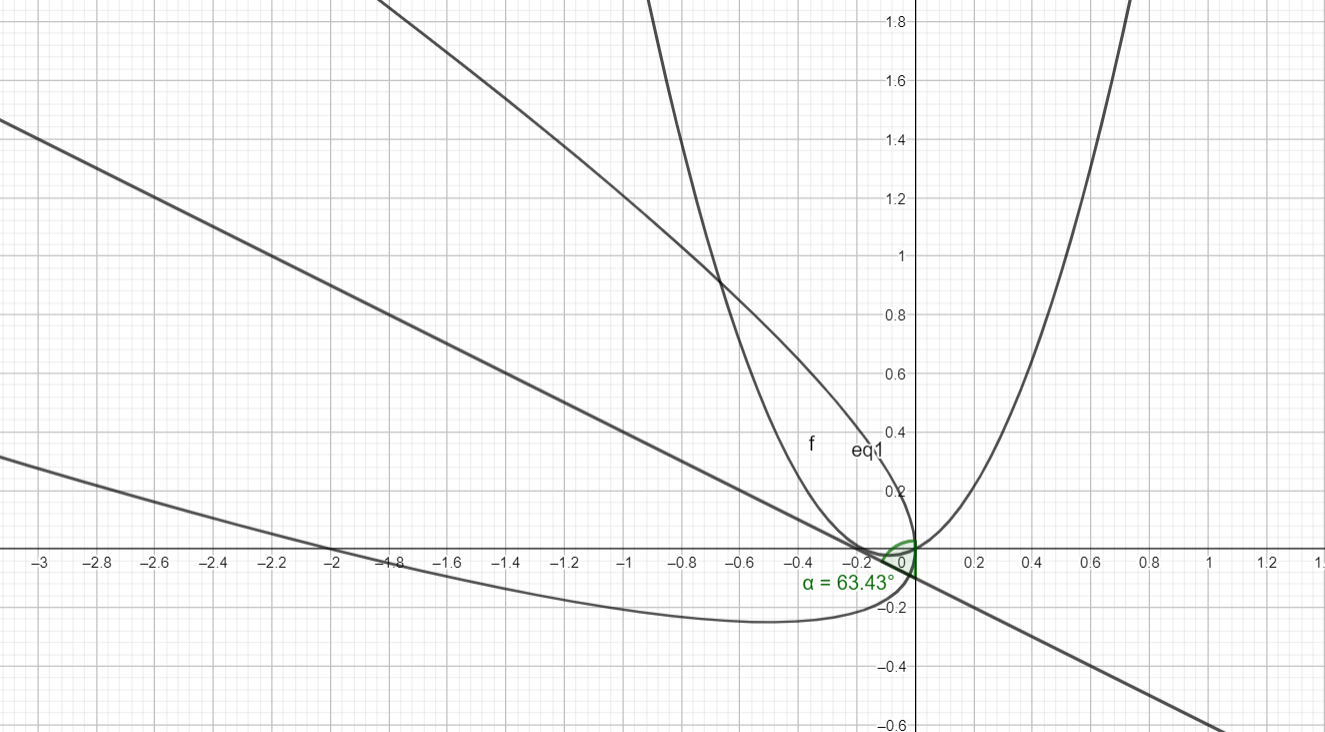
\includegraphics[height=170pt]{Pics/Es1.png}
			\end{center}
			Notare che tutte le informazioni note sulla parabola \virg{di partenza} possono essere trasformate in informazioni sulla parabola \virg{finale}!
			
		\subsubsection{Proposta}
			Per esercitarvi, provate a studiare in questo modo il luogo dei punti dato da:
			\begin{equation*}
				2xy+x+1=0
			\end{equation*}
			si tratta ovviamente di una funzione omografica, studiabile in modo molto più agevole sfruttando la teoria fatta sulle iperboli. Tuttavia, proprio per questa sua natura \virg{facile}, è un ottimo esempio per tenere sott'occhio i vari passaggi del complesso procedimento appena introdotto.
		
	\newpage
	\section{Coniche mediante Eccentricità}
		Tralasciando le motivazioni, che sono comunque intuibili, siamo interessati a studiare la seguente definizione:
		\begin{defin}
			Data una retta $d:\ ax+by+c=0$ ed un punto $F=(p,q)$ chiamiamo \virg{conica} il luogo dei punti $P=(x,y)$ del piano che soddisfano:
			\begin{equation*}
				\frac{\overline{PF}}{\overline{Pd}}=e \qquad \mathrm{per} \quad e\in\R
			\end{equation*} 
		\end{defin}
		dove $\overline{Pd}$ è un abuso di notazione per indicare la distanza del punto $P$ dalla retta $d$. Notiamo subito che, trattandosi di distanze, $e\geq0$. La retta $d$ sarà detta \emph{direttrice} della conica e $F$ \emph{fuoco}.
		
		Ma è lecito chiamare questo oggetto \virg{conica}? Per rispondere a questa domanda dobbiamo assicurarci che, effettivamente, il luogo descritto rappresenti una conica nel senso già precedentemente studiato. Impostiamo i calcoli:
		\begin{equation*}
			\sqrt{(x-p)^2+(y-q)^2}= e\cdot\frac{|ax+by+c|}{\sqrt{a^2+b^2}}
		\end{equation*}
		dalla loro risoluzione otteniamo un'equazione di secondo grado in $x$ e $y$:
		\begin{align} \label{eq:ecc}
			\left[\left(1-e^{2}\right) a^{2}+b^{2}\right] x^{2}+2 a b e^{2} x y+\left[\left(1-e^{2}\right) b^{2}+a^{2}\right] y^{2}-2\left(a^{2} p+b^{2} p+a c e^{2}\right) x + \nonumber \\
			-2\left(a^{2} q+b^{2} q+b c e^{2}\right) y+\left(p^{2}+q^{2}\right)\left(a^{2}+b^{2}\right)-c^{2} e^{2}=0
		\end{align}
		Ma per quanto detto prima ogni equazione di questo tipo è interpretabile come una conica nel piano, quindi il nome è lecito. Inoltre notiamo che ci sarà sempre almeno un punto del piano che appartiene a questo luogo geometrico, quale?
		
		Adesso che abbiamo una definizione alternativa di coniche, siamo interessati, come prima, a classificarle. Di più: siamo interessati a vedere se la loro classificazione dipende dal parametro $e$. Calcoliamo il determinante di $M_2$.
		\begin{equation*}
			\mathrm{det}(M_2) = \mathrm{det}\left(
			\begin{array}{cc}
				\left(1-e^{2}\right) a^{2}+b^{2} & abe^2 \\
				abe^2 & \left(1-e^{2}\right) b^{2}+a^{2}
			\end{array} \right) = (1-e^2)\cdot(a^2 + b^2)^2
		\end{equation*}
		\Egrave evidente che il segno di questo determinante dipenda solo dal fattore $(1-e^2)$, infatti $a$ e $b$ non possono essere contemporaneamente nulli. In particolare:
		\begin{equation*}
			\left\{
			\begin{array}{ll}
				\mathrm{se}\ 0\leq e < 1 & \mathrm{la\ \eqref{eq:ecc}\ individua\ un'ellisse;} \\
				\mathrm{se}\ e=1 & \mathrm{la\ \eqref{eq:ecc}\ individua\ una\ parabola;} \\
				\mathrm{se}\ e>1 & \mathrm{la\ \eqref{eq:ecc}\ individua\ un'iperbole.}
			\end{array} \right.
		\end{equation*}
		\emph{Accipigna}! Possibile che questo parametro $e$ sia l'eccentricità definita tempo fa?
		Proviamo a mostrarlo nel caso di un'ellisse coi fuochi sull'asse delle $x$. In questo caso è evidente che la direttrice sarà della forma $x=k$ con, quindi, $b=0$. Inoltre un tale ellisse si scrive, dalla forma canonica, come:
		\begin{equation*}
			\frac{x^2}{A^2}+\frac{y^2}{B^2}=1 \qquad \allora \qquad B^2x^2 + A^2y^2=A^2B^2 \qquad \mathrm{con} \quad A>B
		\end{equation*}
		Per quanto studiato, la sua eccentricità è:
		\begin{equation*}
			\mathrm{ecc}=\frac{\sqrt{A^2-B^2}}{A}
		\end{equation*}
		che, riferito ai coefficienti delle \eqref{eq:ecc} dove sostituiamo $b=0$, diventa:
		\begin{equation*}
			\mathrm{ecc}=\frac{\sqrt{a^2-(1-e^2)a^2}}{\sqrt{a^2}}=\frac{\sqrt{e^2a^2}}{\sqrt{a^2}}=e
		\end{equation*}
		Allo studente la verifica che l'eccentricità per l'ellisse coi fuochi sull'asse delle $y$ e per le iperboli corrisponde a quella studiata nella teoria.
		Vediamo ora qualche esercizio alla luce della nuova teoria studiata.
		
		\subsubsection{Direttrici di una Conica}
			Ci soffermiamo brevemente sulla questione delle direttrici: sappiamo che definiscono una conica ma ancora non sappiamo, parabola esclusa, come ottenerle e quali siano le formule a partire dall'equazione. Abbiamo quattro casi:
			\begin{enumerate}
				\item ellisse coi fuochi sull'asse delle $x$;
				\item ellisse coi fuochi sull'asse delle $y$;
				\item iperbole coi fuochi sull'asse delle $x$;
				\item iperbole coi fuochi sull'asse delle $y$.
			\end{enumerate}
			Ovviamente non ci occupiamo della parabola in quanto già ampiamente studiata a suo tempo. 
			
			L'idea di base è semplice: poiché per tutte queste coniche conosciamo la formula \emph{esplicita} dell'eccentricità e dei fuochi e sappiamo che sono tutte definite da:
			\begin{equation*}
				\frac{\overline{PF}}{\overline{Pd}}=e
			\end{equation*}
			allora ci basterà imporre $d:\ x=k$ per il primo e terzo caso, $d:\ y=k$ per il secondo e quarto. Questo perché, com'è intuitivo che sia, le direttrici sono perpendicolari alla retta contenente i fuochi.
			Conosciamo $F$, conosciamo $e$ ed abbiamo imposto una formula per $d$, manca da sfruttare un punto \virg{comodo} che ci permetta di fare calcoli semplici: chi se non i vertici? Ovviamente quelli che stanno sulla retta dei fuochi.
			
			Così facendo otteniamo:
			\begin{equation*}
				\left\{
				\begin{array}{ll}
					\displaystyle x=\pm \frac{a^2}{c} & \mathrm{per\ l'ellisse\ e\ l'iperbole\ coi\ fuochi\ sull'asse\ delle\ }x \\ \\
					\displaystyle y=\pm \frac{b^2}{c} & \mathrm{per\ l'ellisse\ e\ l'iperbole\ coi\ fuochi\ sull'asse\ delle\ }y
				\end{array} \right.
			\end{equation*}
			
			\subsection{Esempio pratico}
			
			Mostriamo ora un esempio di come determinare eccentricità, fuochi, direttrici ed assi di simmetria di una conica qualsiasi. Partiamo dall'equazione:
			\begin{equation*}
				22x^2-12xy+17y^2+8x+12y-4=0
			\end{equation*}
			\Egrave evidente che dovremo \virg{tornare indietro} fino alla forma canonica, determinarne quanto richiesto e \virg{riportarlo avanti}.
			\begin{itemize}
				\item Poiché, come detto, dovremo tornare alla forma canonica, non ha senso calcolare ora il determinante di $M_3$. Potremmo evitare di calcolare anche il determinante di $M_2$, ma lo facciamo ugualmente dato che ci torna utile.
				\begin{equation*}
					\mathrm{det}(M_2)=\mathrm{det}\left(
					\begin{array}{cc}
						22 & -6 \\
						-6 & 17
					\end{array} \right) = 374-36=338>0 \quad \allora \quad \mathrm{è\ un'ellisse.}
				\end{equation*}
				\item Calcoliamo gli autovalori di $M_2$:
				\begin{align*}
					\mathrm{det}\left(
					\begin{array}{cc}
						22-\lambda & -6 \\
						-6 & 17-\lambda
					\end{array} \right) = 0 \quad \allora \quad (22-\lambda)(17-\lambda)-36=0 \\ \quad \allora \quad \lambda^2-39\lambda+338=0
				\end{align*}
				i due autovalori sono $\lambda_1=13$ e $\lambda_2=26$. Notare che nell'equazione di secondo grado appena scritta, il termine noto è il determinante di $M_2$.
				\item Con calcoli analoghi a quelli fatti nell'esercizio \ref{sub:sec1}, otteniamo gli autovalori normalizzati:
				\begin{equation*}
					\overrightarrow{v_1^{*}}=\left(\frac{2}{\sqrt{13}},\frac{3}{\sqrt{13}}\right) \quad \mathrm{per} \ y=\frac{3}{2}x \quad \mathrm{e} \quad \overrightarrow{v_2^{*}}=\left(-\frac{3}{\sqrt{13}},\frac{2}{\sqrt{13}}\right) \quad \mathrm{per} \ y=-\frac{2}{3}x
				\end{equation*}
				come al solito notiamo che i due autovettori individuano direzioni perpendicolari: esattamente quelle degli assi di simmetria dell'ellisse! \emph{Questo è uno strumentopolo che ci servirà più tardi}.
				\item Dalla rotazione:
				\begin{equation*}
					\mathrm{R:}\ \left\{
					\begin{array}{l}
						x_n = \displaystyle \frac{2}{\sqrt{13}} x_v - \frac{3}{\sqrt{13}} y_v \\ \\
						y_n = \displaystyle \frac{3}{\sqrt{13}} x_v + \frac{2}{\sqrt{13}} y_v
					\end{array} \right.
				\end{equation*}
				ottengo l'equazione:
				\begin{equation*}
					13x^2+26y^2+4\sqrt{13}x-4=0
				\end{equation*}
				Poiché necessito di portarla in forma canonica per utilizzare le formule note, devo completare il quadrato ed ottenere $1$ a destra dell'uguale:
				\begin{align*}
					\quad &\allora \quad 13\left(x^2+\frac{4}{\sqrt{13}}x+\left(\frac{2}{\sqrt{13}}\right)^2-\frac{4}{13}\right)+26y^2-4=0 \\ 
					\quad &\allora \quad 13\left(x+\frac{2}{\sqrt{13}}\right)^2+26y^2=8 \\
					\quad &\allora \quad \frac{\left(x+\frac{2}{\sqrt{13}}\right)^2}{\left(\frac{8}{13}\right)}+\frac{y^2}{\left(\frac{8}{26}\right)}=1 \\
					\quad &\allora \quad \frac{x^2}{\left(\frac{8}{13}\right)}+\frac{y^2}{\left(\frac{8}{26}\right)}=1 \\
				\end{align*}
				questo è stato possibile imponendo la traslazione:
				\begin{equation*}
					\mathrm{T:}\ \left\{
					\begin{array}{l}
						x_n + \frac{2}{\sqrt{13}} = x_v \\
						y_n = y_v
					\end{array} \right. \qquad \allora \qquad
					\mathrm{T:}\ \left\{
					\begin{array}{l}
						x_n = x_v - \frac{2}{\sqrt{13}} \\
						y_n = y_v
					\end{array} \right.
				\end{equation*}
				dove ciò che sta dopo la traslazione: $ \left(x + \frac{2}{\sqrt{13}}\right)$ è posto uguale a ciò che c'era prima. Dopodiché è stata riordinata.
			\end{itemize}
			Ho ottenuto l'equazione canonica di un'ellisse reale. Noto che $a^2>b^2$ quindi sarà un ellisse reale con i fuochi sull'asse delle $x$. Questa informazione è essenziale nel determinare le caratteristiche richieste dall'esercizio.
			\begin{itemize}
				\item Calcolo l'eccentricità:
				\begin{equation*}
					e=\frac{\sqrt{a^2-b^2}}{a}=\frac{\displaystyle \frac{2}{\sqrt{13}} }{\displaystyle \sqrt{\frac{8}{13}} }= \frac{1}{\sqrt{2}}
				\end{equation*}
				questa, essendo un rapporto tra distanze, non viene alterata dalle isometrie individuate.
				\item Determino i fuochi:
				\begin{align*}
					\begin{array}{c}
						\displaystyle F_1=\left( \frac{2}{\sqrt{13}}, 0 \right) \quad \stackrel{\mathrm{T}}{\allora} \quad F_1=\left( 0 , 0 \right) \quad \stackrel{\mathrm{R}}{\allora} \quad F_1=\left( 0 , 0 \right)
						\\
						\\
						\displaystyle F_2=\left(\displaystyle -\frac{2}{\sqrt{13}}, 0 \right) \quad \stackrel{\mathrm{T}}{\allora} \quad F_2=\left( -\frac{4}{\sqrt{13}}, 0 \right) \quad \stackrel{\mathrm{R}}{\allora} \quad F_2=\left( -\frac{8}{13}, -\frac{12}{13} \right)
					\end{array}
				\end{align*}
				dove, per determinare la \virg{versione} successiva, abbiamo preso le coordinate prima delle trasformazioni (considerandole quindi \virg{vecchie}) e le abbiamo sostituite nei sistemi $T$ ed $R$ per ottenere le loro controparti \virg{nuove}.
				\item Determino le direttrici notando che i fuochi sono sull'asse delle $x$:
				\begin{align*}
					x=\pm \frac{a^2}{c} = \pm \frac{4}{\sqrt{13}} \quad \stackrel{\mathrm{T}}{\allora} \quad x=\pm \frac{4}{\sqrt{13}} - \frac{2}{\sqrt{13}} \ 
					\begin{array}{c}
						\rotatebox{35}{$\longrightarrow$} \\
						\rotatebox{-35}{$\longrightarrow$}
					\end{array} 
					\begin{array}{l}
						\displaystyle x=\frac{2}{\sqrt{13}} \ (\star)\\ \\
						\displaystyle x=-\frac{6}{\sqrt{13}} \ (\diamond)
					\end{array}
				\end{align*}
				adesso andrebbero ruotate. Ma mi accorgo che prima devo invertire la rotazione: devo essere in grado di sostituire alle variabili qui presenti (quelle \virg{vecchie}) le variabili \virg{nuove}. Per poterlo fare devo aver scritte le prime in funzione delle seconde, ma per ora ho solo il contrario. L'idea è di invertire il sistema $R$ usando il metodo di riduzione. Lo svolgimento non è immediato ma vediamone qualche passaggio intermedio:
				\begin{align*}
					\mathrm{R} \quad &\allora \quad 
					\begin{array}{r}
						\displaystyle \frac{3}{2}(1)-(2): \\ \\
						\displaystyle (1)+\frac{3}{2}(2):
					\end{array}
					\left\{
					\begin{array}{l}
						\displaystyle \frac{3}{2}x_n - y_n = -\frac{3}{2}\frac{3}{\sqrt{13}} y_v - \frac{2}{\sqrt{13}} y_v \\ \\
						\displaystyle x_n + \frac{3}{2}y_n = \frac{2}{\sqrt{13}} x_v + \frac{3}{2}\frac{3}{\sqrt{13}} x_v
					\end{array} \right. \\ \\
					\quad &\allora \quad 
					\left\{
					\begin{array}{l}
						\displaystyle \frac{3}{2}x_n - y_n = -\frac{13}{2\sqrt{13}} y_v \\ \\
						\displaystyle x_n + \frac{3}{2}y_n = \frac{13}{2\sqrt{13}} x_v
					\end{array} \right. \\ \\
					\quad &\allora \quad 
					\mathrm{R}^{-1}:\ \left\{
					\begin{array}{l}
						\displaystyle x_v = \frac{2\sqrt{13}}{13}x_n + \frac{3\sqrt{13}}{13}y_n \\ \\
						\displaystyle y_v = \frac{2\sqrt{13}}{13}y_n - \frac{3\sqrt{13}}{13}x_n
					\end{array} \right.
				\end{align*}
				uso ciò che ho ottenuto per ruotare le direttrici $(\star)$ e $(\diamond)$:
				\begin{align*}
					(\star) \quad &\allora \quad \frac{2}{\sqrt{13}}=\frac{2\sqrt{13}}{13}x + \frac{3\sqrt{13}}{13}y \quad \allora \quad 2x+3y=2 \\ \\
					(\diamond) \quad &\allora \quad -\frac{6}{\sqrt{13}}=\frac{2\sqrt{13}}{13}x + \frac{3\sqrt{13}}{13}y \quad \allora \quad 2x+3y=-6
				\end{align*}
				viste tutte le considerazioni sugli autovettori, la \emph{bella} equazione delle direttrici non dovrebbe sorprenderci.
				\item Determino gli assi di simmetria. Potrei applicare lo stesso procedimento che ho usato per le direttrici agli assi delle $x$ e delle $y$ e otterrei quanto desiderato. Tuttavia questo procedimento è vantaggioso solo quando ho gia invertito la rotazione. Altrimenti conviene determinare il centro di simmetria e far passare da lì due rette con le direzioni individuate dagli autovettori. Per il centro di simmetria ho due possibilità: trasformo l'origine oppure calcolo il punto medio del segmento che ha come estremi i fuochi \virg{finali}. In entrambi i casi otterrò il punto $P=\left( -4/13, -6/13 \right)$ e farò passare per questo due rette di coefficiente rispettivamente $m_1=3/2$ e $m_2=-2/3$. Ottengo:
				\begin{equation*}
					2x+3y=-2 \qquad \mathrm{e} \qquad 3x-2y=0
				\end{equation*}			
			\end{itemize}
			
		\subsection{Spunti di Riflessione}
			Mi pongo ora un problema: è possibile che sia necessario tutto questo procedimento in casi in cui, magari, data un'eccentricità, un fuoco ed una direttrice mi viene chiesto di determinare soltanto l'altro fuoco e l'altra direttrice (ammesso che esistano)?
			Esaminiamo il caso dell'ellisse coi fuochi sull'asse delle $x$, per gli altri vi invito a riflettere autonomamente.
			Un'idea può essere quella di determinare la distanza tra la direttrice e il fuoco, ricostruire se possibile la distanza focale e quindi poi ottenere l'altra direttrice.
			
			La distanza tra le direttrici è $\displaystyle 2\frac{a^2}{c}$, la distanza tra i fuochi è $2c$. Da questo segue che la distanza fuoco-direttrice $D_{fd}$ è la metà della differenza di queste due grandezze:
			\begin{equation*}
				D_{fd}= \frac{1}{2}\left( 2\frac{a^2}{c} - 2c \right) = \frac{1}{2}\frac{2a^2-2c^2}{c}=\frac{a^2-c^2}{c}
			\end{equation*}
			ricordandoci che l'eccentricità è $e=a/c$:
			\begin{equation*}
				=\frac{a^2-c^2}{c} = \frac{a}{e}-e\cdot a = a\left( \frac{1}{e}-e \right)= a\left( \frac{1-e^2}{e} \right)=D_{fd}
			\end{equation*}
			ma se $c=e\cdot a$ allora mi basta ricavare $a$ dall'equazione appena ottenuta per ottenere $c$ in funzione di solo $D_{fd}$ ed $e$:
			\begin{equation*}
				a=D_{fd}{\left( \frac{e}{1-e^2} \right)} \quad \allora \quad c=e\cdot D_{fd}\left( \frac{e}{1-e^2}\right) = D_{fd}\left( \frac{e^2}{1-e^2}\right)
			\end{equation*}
			ma $D_{fd}$ può essere calcolata anche come distanza punto-retta sui dati del problema. Quindi siamo riusciti a scrivere la semidistanza focale in funzione solo dei dati del problema, che non richiedono di portare la conica in forma canonica. Sapendo poi le distanze si preservano nelle rototraslazioni, mi resta da calcolare la retta che contiene i fuochi per aver concluso. Ma è facile! \Egrave la perpendicolare alla direttrice passante per il fuoco dato! 
			
			Di più: a metà strada tra i due fuochi si trova il centro di simmetria. Uno dei due assi è la retta per i fuochi, l'altro è la perpendicolare passante per quel centro. 
			
			Ancora di più: ora che ho gli assi posso metterli a sistema con l'equazione della conica ottenuta dai dati, in questo modo determino i vertici. Ma una volta che ho i vertici e gli assi di simmetria rappresentare una conica è un giochetto! \par
			\vspace{18pt}
			\begin{center}
				\emph{\Egrave utile tutto ciò? Boh, forse. Però è figo!}
			\end{center}
\end{document}